\chapter{Threshold-Issued, Sybil-Resistant Private Identity System from Anonymous Credentials and Nullifiers}\label{chap5}

\section{Introduction}\label{sec:threshold-intro}
Self-sovereign identity (SSI) systems enable users to control their digital identities with strong privacy, Sybil resistance, and minimal issuer interaction. Distributing trust across multiple issuers is critical to avoid single points of failure. CanDID~\cite{maram_candid_2020} is a pioneering SSI system that uses multi-party computation (MPC) to deduplicate identities and issue credentials via a (threshold) committee of signing nodes. While effective, it has drawbacks: slow MPC-based deduplication, frequent issuer interactions, linkability risks, and little protection for credential non-transferability. Similar to Coconut~\cite{sonnino_coconut_2020}, a threshold credential system that distributes trust across multiple issuers, T-SIRIS employs a $t$-out-of-$N$ threshold issuance model to enhance decentralization. However, Coconut lacks a mechanism to prevent sybil attacks, a critical requirement for self-sovereign identity (SSI) systems. T-SIRIS addresses this gap by integrating anonymous, deterministic nullifiers from our Credential Relationship Binding Nullifier (CRBN) scheme (Chapter~\ref{chap4}), adding just 2.49ms to issuance overhead to credential issuance (Section~\ref{sec:threshold-performance}) while ensuring users cannot obtain multiple credentials per context. Our work extends the model in CanDID and answers open questions. 



This chapter presents T-SIRIS, a threshold Sybil-resistant identity system built on our multi-issuer multi-credential anonymous credential system (MIMC-ABC) from Chapter~\ref{chap3} and Credential Relationship Binding Nullifier (CRBN) from Chapter~\ref{chap4}. T-SIRIS uses a $t$-out-of-$N$ threshold issuance model, secure against $t-1$ malicious issuers. We compare T-SIRIS with CanDID and S3ID~\cite{rabaninejad_attribute-based_2024}, which uses threshold anonymous counting tokens (tACT), showing improvements in efficiency and functionality. My implementation can be found on GitHub\footnote{https://github.com/sampolgar/t-siris}


\subsection*{Chapter Roadmap}
The remainder of this chapter is structured as follows: Section \ref{chap5:sec_preliminaries} covers cryptographic preliminaries. Section \ref{chap5:sec_tsiris} presents the T-SIRIS system model and security requirements. Section \ref{chap5:ourconstruction} details our construction and protocols. Section \ref{chap5:sec_perf_eval} evaluates our performance against state-of-the-art alternatives.

\subsection{Motivation and Challenges}

Traditional Attribute-Based Anonymous Credential systems (ABCs) are based on a centralized issuer, which has its own security flaws - a malicious issuer can issue credentials that can't be traced in an anonymous system, undermining the system's integrity. To address this, we distribute security among $N$ nodes, requiring a threshold of at least $t$ nodes to issue a valid credential. 

CanDID~\cite{maram_candid_2020} pioneered Sybil-resistant identity with legacy credential oracles, but relies on costly multi-party computation (MPC) among committee nodes for deduplication and requires interactive issuance for context credentials, contradicting self-sovereign principles. Each transaction requires communication with committee members, introducing privacy vulnerabilities where a single malicious node can link different user transactions.

\subsubsection*{CanDID}
CanDID deduplicates a user attribute, e.g. social security number using MPC, storing a unique value in a table $T_{\text{Dedup}}$. Users create a master credential from legacy data via oracles, then request context-specific credentials. Its limitations include:

\begin{itemize}
    \item \textbf{Deduplication:} MPC deduplication is slow and reveals a pseudonym to issuers, enabling pseudonym linking. T-SIRIS uses CRBN, computing a nullifier $y = g^{1/(s + \text{ctx})} \in \mathbb{G}_1$ with user key $k \in \mathbb{Z}_p$ and context $\text{ctx}$. This is anonymous and many times faster than tACT~\cite{rabaninejad_attribute-based_2024} (see Section~\ref{chap5:sec_perf_eval}).

    \item \textbf{Efficient Deduplication and Verification:} T-SIRIS achieves fast deduplication using CRBN, computing a nullifier $y = g^{1/(s + \text{ctx})} \in \mathbb{G}_1$ with user key $k \in \mathbb{Z}_p$ and context $\text{ctx}$. Unlike Coconut~\cite{sonnino_coconut_2020}, which lacks sybil resistance, and CanDID’s MPC-based deduplication, CRBN is pairing-free and $5\times$ faster than S3ID’s tACT~\cite{rabaninejad_attribute-based_2024}. Verification scales sublinearly with attributes $n$, achieving up to $44.1\times$ speedup over tACT for $n=64$ (see Section~\ref{chap5:sec_perf_eval}).
    
    \item \textbf{Context Credential Issuance:} CanDID requires issuer interaction for each context credential, e.g., ``over 18.’’ T-SIRIS users receive credentials from different issuers and use ZKPs to prove predicates $\phi(\vec{m}) = m_1 \geq 18$ based on the attributes in their set of credentials, allowing flexibility and dynamic verification scenarios without interacting with an issuer each time. 
    
    \item \textbf{Sybil Resistance:} CanDID tracks public keys, risking linkability. T-SIRIS embeds $s$ in all credentials, using CRBN with ZKP $\Pi^{\mathcal{R}_{\text{null}}} = \text{ZKPoK}\{(k): y = g^{1/(s + \text{ctx})}\}$ for unlinkable Sybil resistance.
\end{itemize}

Both systems use a master-context credential hierarchy, but T-SIRIS allows different issuers for context credentials and supports flexible ZKP-based predicates.

\subsubsection*{S3ID/tACT} \cite{rabaninejad_attribute-based_2024} uses tACT, based on Shacham-Waters signatures, for Sybil resistance and threshold issuance. Both T-SIRIS and S3ID embed a user key $s$ in credentials. T-SIRIS improves in:
\begin{itemize}
    \item \textbf{Efficiency:} Our verification is nearly constant as the number of attributes in signatures increases due to efficient Schnorr signatures and Multi-Scalar Multiplication techniques, offering up to $44.1\times$ faster verification for $n=64$ attributes (see Section~\ref{chap5:sec_perf_eval}).
    \item \textbf{Predicate Support:} S3ID’s Groth-Sahai proofs limit predicate expressiveness or trade expressiveness for efficiency. T-SIRIS’s MIMC-ABC supports complex computation over group exponents with efficient Schnorr proofs.
\end{itemize}


\subsubsection*{Managing SSI Features with Privacy Preserving Cryptography}
SSI requires unlinkability, Sybil resistance, and efficiency. Approaches include tokens (tACT~\cite{rabaninejad_attribute-based_2024}), zkSNARKs~\cite{rosenberg_zk-creds_2022}, and anonymous credentials (ABC). T-SIRIS’s ABC-based design with CRBN and MIMC-ABC balances speed and flexibility, scaling well with attributes $n$ and issuers $N$.


\subsection{Contributions}
\label{sec:tsiris_contributions}

Our Threshold Sybil-Resistant Identity System (T-SIRIS) advances self-sovereign identity (SSI) by combining efficiency, expressiveness, and security in a multi-issuer setting. Built on the Multi-Issuer Multi-Credential Anonymous Credential system (MIMC-ABC) from Chapter~\ref{chap3} and the Credential Relationship Binding Nullifier (CRBN) from Chapter~\ref{chap4}, T-SIRIS outperforms existing systems like CanDID~\cite{maram_candid_2020} and S3ID~\cite{rabaninejad_attribute-based_2024}. Below, we outline our contributions, aligning them with S3ID’s claims to highlight T-SIRIS’s improvements.

\begin{enumerate}
    \item \textbf{Efficient Deduplication and Verification:} T-SIRIS achieves fast deduplication using CRBN, computing a nullifier $y = g^{1/(s + \text{ctx})} \in \mathbb{G}_1$ with user key $s \in \mathbb{Z}_p$ and context $\text{ctx}$. Unlike Coconut~\cite{sonnino_coconut_2020}, which lacks sybil resistance, and CanDID’s MPC-based deduplication, CRBN is pairing-free and many times faster than S3ID’s tACT~\cite{rabaninejad_attribute-based_2024}. Verification scales sublinearly with attributes $n$, achieving up to $44.1\times$ speedup over tACT for $n=64$ 
    
    \item \textbf{Expressive Predicate Proofs:} T-SIRIS supports complex predicates (e.g., $\phi(\vec{m}) = m_1 \geq 18 \wedge m_2 \in S$) via MIMC-ABC and Schnorr-based zero-knowledge proofs (ZKPs). Unlike S3ID’s Groth-Sahai proofs, which limit expressiveness, T-SIRIS enables range proofs and set membership with sublinear complexity, enhancing flexibility for SSI applications (see Chapter~\ref{chap6}).
    
    \item \textbf{Provably Secure SSI:} T-SIRIS provides formal security definitions and proofs for unforgeability, Sybil resistance, strong unlinkability, and identity binding, secure against $t-1$ malicious issuers in a $t$-out-of-$N$ threshold model. Our proofs, based on the $q$-DDHI assumption for CRBN and SDLP for MIMC-ABC, extend S3ID’s tACT-based security to multi-issuer settings with identity binding (see Section~\ref{chap3}).
    
    \item \textbf{Non-transferability and Identity Binding:} T-SIRIS embeds a user identifier $\id$ in all credentials, ensuring only the owner can use them, similar to S3ID. 
\end{enumerate}

\textbf{Comparison with S3ID/tACT:} S3ID~\cite{rabaninejad_attribute-based_2024} claims efficient deduplication, non-interactive credential generation, unlinkability, and non-transferability using tACT. T-SIRIS achieves these with superior efficiency and expressiveness (Schnorr vs. Groth-Sahai). While S3ID supports single-issuer deduplication, T-SIRIS’s MIMC-ABC enables multi-issuer identity binding, addressing a broader range of SSI use cases. Both systems ensure non-transferability via a private key, but T-SIRIS’s ZKP $\Pi^{\mathcal{R}_{\text{null}}} = \text{ZKPoK}\{(k): y = g^{1/(s + \text{ctx})}\}$ offers stronger unlinkability against colluding issuers.


\begin{table}[ht]
\centering
\caption{Comparison of T-SIRIS with prior SSI systems.}
\label{tab:comparison-chap5}
\begin{tabular}{l|cccccc}
\toprule
\textbf{System} & \textbf{Sybil Resist.} & \textbf{Threshold} & \textbf{Non-Interact.}$^{\dagger}$ & \textbf{Non-Transfer.}$^{\ddagger}$ & \textbf{Complex Pred.}$^{\S}$ & \textbf{M.I. Anon.}$^{\P}$ \\
\midrule
CanDID~\cite{maram_candid_2020} & \ding{51}$^{\text{a}}$ & \ding{51} & \ding{55} & \ding{55} & \ding{55} & \ding{55} \\
SyRA~\cite{crites_syra_2024} & \ding{51} & \ding{55} & \ding{51} & \ding{55} & \ding{55} & \ding{55} \\
S3ID~\cite{rabaninejad_attribute-based_2024} & \ding{51} & \ding{51} & \ding{51} & \ding{51} & \ding{55} & \ding{55} \\
Coconut~\cite{sonnino_coconut_2020} & \ding{55} & \ding{51} & \ding{51} & \ding{51} & \ding{51} & \ding{55} \\
T-SIRIS (Ours) & \ding{51} & \ding{51} & \ding{51} & \ding{51} & \ding{51} & \ding{51} \\
\bottomrule
\end{tabular}
\begin{flushleft}
\footnotesize
$^{\dagger}$ Non-interactive application credential generation i.e. verify against predicates from multiple credentials \\
$^{\ddagger}$ Credentials bound to the true owner (Section~\ref{chap5:ourconstruction}). \\
$^{\S}$ Support for complex predicates, e.g., range proofs (Section~\ref{sec:chap5-threshold-security}). \\
$^{\P}$ Anonymity against malicious issuers (Section~\ref{subsec:malicious_issuer_security_guarantee}). \\
$^{\text{a}}$ Pseudonymous, not fully anonymous. \\
\textit{Note:} We compare with CanDID for its SSI prominence, SyRA for its VRF-based Sybil resistance, S3ID for its threshold similarity, and Coconut for its threshold issuance baseline.
\end{flushleft}
\end{table}







\section{Preliminaries}\label{chap5:sec_preliminaries}

\begin{definition}[Shamir Secret Sharing]
A $(t,n)$ secret sharing scheme $\mathsf{SS}$ consists of the following $\PPT$ algorithms over message space $\mathcal{X}$:
\begin{itemize}
    \item $\mathsf{Share}(1^{\lambda}, t, n, x) \to ([x]_1, \dots, [x]_n):$ Takes security parameter $\lambda$, threshold $t$, number of parties $n$, and secret $x \in X$. Outputs $n$ shares $([x]_1, \dots, [x]_n)$.
    
    \item $\mathsf{Combine}([x]_{i_1}, \dots, [x]_{i_t}) \to x:$ Takes as input $t$ distinct shares $[x]_{i_j}$ where $i_j \in [n]$ for $j \in [t]$, and outputs the reconstructed secret $x \in \mathcal{X}$.
\end{itemize}
\end{definition}




\subsection{Threshold Rerandomizable Signature}

Our base-building block is the threshold PS signature scheme from \cite{tomescu_utt_2022} using Shamir secret sharing with similarities to \cite{sonnino_coconut_2020} to distribute trust among multiple issuers. The key pair $(\mathsf{sk}, \mathsf{vk})$ is $(t,n)$-secret-shared among the signers, where each signer $i$ holds a share secret key $\mathsf{sk}_i$ and a share verification key $\mathsf{vk}_i$. This enables subsets of at least $t+1$ signers to collaboratively produce a signature that verifies under the combined verification key $\mathsf{vk}$, while ensuring that no subset of $t$ or fewer signers can forge signatures.

We assume up to $t-1$ malicious issuers in an $n$-issuer system, where $t$ is the threshold, reflecting realistic collusion scenarios in decentralized settings. The adversary cannot break the hard problems our schemes are built upon, and network conditions support standard threshold protocols. Similar to Coconut’s threshold issuance~\cite{sonnino_coconut_2020}, our threshold PS signature scheme distributes trust among $n$ issuers using Shamir secret sharing. However, we extend this foundation by integrating nullifiers from Chapter~\ref{chap4}, enabling sybil resistance—a critical feature for identity systems that Coconut does not address.

Importantly, this threshold construction distributed trust among multiple issuers while preserving the core properties of our underlying building block PS signature scheme - unforgeability and rerandomizability. Additionally, the end-signature algebraic structure is the same, and therefore, the verification algorithm and proof system compatibility are the same.


\begin{definition}[PS Threshold Signatures over Pedersen Commitments]
A PS threshold signature scheme $\mathsf{RS}$ over Pedersen commitments consists of the following algorithms:
\begin{itemize}
    \item $\mathsf{DistKeyGen}(1^{\lambda}, t+1, n, \ell) \to (\mathsf{ck}, \mathsf{vk}, (\mathsf{sk}_i, \mathsf{vk}_i)_{i \in [n]}):$ Takes security parameter $\lambda$, corruption threshold $t$, number of parties $n$, and attribute count $\ell$. Outputs commitment key $\mathsf{ck}$, verification key $\mathsf{vk}$, and per-party keys $(\mathsf{sk}_i, \mathsf{vk}_i)$.
    
    \item $\mathsf{ShareSign}(\mathsf{ck}, \mathsf{sk}_i, (\mathsf{cm}_k, \pi_k^{\mathsf{zkpok}})_{k \in [\ell]}; h) \to [\sigma^*]_i:$ Takes party $i$'s secret key $\mathsf{sk}_i$, commitments $\mathsf{cm}_k$ with ZK proofs $\pi_k^{\mathsf{zkpok}}$, and randomizer $h$. Outputs signature share $[\sigma^*]_i$.
    
    \item $\mathsf{ShareVer}(\mathsf{ck}, \mathsf{vk}_i, (\mathsf{cm}_k, \pi_k^{\mathsf{zkpok}})_{k \in [\ell]}, [\sigma^*]_i; h) \to \{0,1\}:$ Takes party $i$'s verification key $\mathsf{vk}_i$, commitments with proofs, and signature share $[\sigma^*]_i$. Outputs accept ($1$) or reject ($0$).
    
    \item $\mathsf{Aggregate}(\mathsf{ck}, \{[\sigma^*]_i\}_{i \in S}, \{r_k\}_{k \in [\ell]}) \to \sigma:$ Takes signature shares from subset $S$ of parties and commitment randomness values. Outputs aggregated signature $\sigma$.

    \item $\mathsf{Rerand}(\mathsf{vk}, \sigma, \Delta_r, \Delta_u) \rightarrow \sigma'$: Creates a rerandomized signature $\sigma'$ from signature $\sigma$ using randomization values $\Delta_r, \Delta_u$.
    
    \item $\mathsf{Verify}(\mathsf{vk}, \mathsf{cm}, \sigma) \rightarrow \{0,1\}$: Verifies signature $\sigma$ on commitment $\mathsf{cm}$ using public key $\mathsf{vk}$.
    
\end{itemize}
\end{definition}




\subsubsection{Construction}\label{threshold-ps-construction}


Our threshold PS construction works as follows:
A user with attributes $\attrs = [m_1, \ldots, m_\ell]$ generates a commitment $\cm = \CMCom([\attrs];r)$. The user interacts with signers using a pre-agreed random element $h \in \G_1$, alternatively, \cite{sonnino_coconut_2020} generates this with a hash-to-group of the commitment $h \gets \mathcal{H}(\cm)$. The user sends $\cm$ with $\pircom$ proving its opening to each signer. Signers verify the proof and return a signature share $[\sigma^*]_i = \mathsf{tPSutt.ShareSign}(\ck, \mathsf{sk}_i, (\mathsf{cm}_k, \pircom_k); h)$. The user verifies each share and checks the consistency of the message and proof previously shared $\mathsf{tPSutt.ShareVer}(\ck, \mathsf{vk}_i, (\mathsf{cm}, \pi^{\mathsf{zkpok}}), [\sigma^*]_i; h)$. The user identifies a set $S$ of at least $t+1$ valid shares and aggregates them, outputting their signature $\sigma \leftarrow \mathsf{tPSutt.Aggregate}(\ck, ([\sigma^*]_i)_{i \in S}, r)$ which verifies under the combined  verification key $\mathsf{PSutt.Ver}(\mathsf{vk}, \mathsf{cm}, \sigma) = 1$.


\begin{itemize}
    \item $\mathsf{tDistKeyGen}(1^{\lambda}, t+1, n, \ell) \to (\ck, \vk, h, (\mathsf{sk}_i, \mathsf{vk}_i)_{i \in [n]}):$ Takes input the security parameter, $t$ the corruption threshold, $n$ is number of nodes, $\ell$ is the credential message length. Outputs $\ck, \vk$ the commitment and verification keys generated with the secrets and $\sk_i, \vk_i$ the shared keys to distribute to $n$ nodes. let $\mathcal{X}$ and $\psi_k $ be $t$ degree polynomials:
    \begin{itemize}
        \item For the shared $x$ value: $\mathcal{X} \sample \Z_p[X], x \gets \mathcal{X}(0)$, $\{[x]_i \gets \mathcal{X}(i)\}_{i\in [n]}$
        \item For the shared $u$ value: $\mu \sample \Z_p[X], h \gets \mu(0)$, $\{[h]_i \gets \mu(i)\}_{i\in [n]}$
        \item For the $s$ shared $y$ values: $\{\psi_k \sample \Z_p[X], y_k \gets \psi_k(0)\}_{k \in [\ell]}$, $\{[y_k]_i \gets \psi_k(i)\}_{k \in [\ell], i \in [n]}$
        \item using the secret, non-shared values, trusted setup party computes $\vk \gets \tilde{g}^x, h \gets g^u, \ck \gets \CMSetup(1^{\lambda}, \ell, \vec{y})$ and parses $\ck$ as $(g, \vec{g}, \tilde{g}, \vec{\tilde{g}})$. Note that $g_k = g^{y_k}, \tilde{g}_k = \tilde{g}^{y_k}$
        \item computes shared secret values $\{\sk_i \gets ([x]_i, ([y_k]_i))_{k\in[\ell]}\}_{i \in [n]}, \{\vk \gets (\tilde{g}^{[x]_i}, (\tilde{g}^{[y_k]_i})_{k\in[\ell]})\}_{i \in [n]}$
        \item $\mathsf{Return } $ $ \ck, \vk, \{\sk_i, \vk_i\}_{i \in [n]}$
    \end{itemize}

    \item $\mathsf{tPrepare}(\ck, h, \attrs) \to (\{\cm_k, \Pi^{\mathcal{R}_{\mathsf{com}}}(\cm_k, m_k, r_k)\}_{k \in [\ell]}, h):$ User commits to each $m$ individually: 
    \begin{itemize}
        \item Samples $\{r_k\}_{k \in |\ell|} \sample \Z_p^*$
        \item Computes $\cm_k = h^{m_k}g^{r_k}$ and generates proofs for each $\{\cm_k = \Pi^{\mathcal{R}_{\mathsf{com}}}(\cm_k, m_k, r_k)\}_{k \in |\ell|}$
    \end{itemize}

    \item $\mathsf{tShareSign}(\ck, \mathsf{sk}_i, \{\cm_k, \pi_k^{\mathsf{zkpok}}\}_{k \in [\ell]}, h) \to [\sigma^*]_i:$ the user runs $\mathsf{tShareSign}$ with at least $t$ nodes. 
    \begin{itemize}
        \item Signer parses $g$ from $\ck$ and verifies $\{\ZKVerify(\Pi^{\mathcal{R}_{\mathsf{com}}}(\cm_k, m_k, r_k))\}_{k \in [\ell]}$
        \item Signer parses $\sk_i$ as $[x]_i, \{[y_k]_i\}_{k \in [\ell]}$
        \item Signer signs their share $[\sigma^*]_i \gets (h, h^{[x]_i} \prod_{k \in [\ell]} \cm_k^{[y_k]_i} )$ = $(h, h^{[x]_i + \sum_{k \in [\ell]} m_k[y_k]_i} \cdot g^{\sum_{k \in [\ell]} r_k [y_k]_i})$
    \end{itemize}
    
    \item $\mathsf{tShareVer}(\ck, \mathsf{vk}_i, \{\cm_k, \pi_k^{\mathsf{zkpok}}\}_{k \in [\ell]}, [\sigma^*]_i; h) \to \{0,1\}:$ Run by a user to verify the signed share returned from each node before aggregating together. 
    \begin{itemize}
        \item Parse $[\sigma^*]_i$ as $([\sigma^*]_{i,1}, [\sigma^*]_{i,2})$ and check $h = [\sigma^*]_{i,1}$. 
        \item Verifies $\{\ZKVerify(\Pi^{\mathcal{R}_{\mathsf{com}}}(\cm_k, m_k, r_k))\}_{k \in [\ell]}$
        \item Parses $\vk_i$ as $(\tilde{g}^{[x]_i}, \{\tilde{g}^{[y_k]_i}\}_{k \in [\ell]})$
        \item Asserts $e([\sigma^*]_{i,2}, \tilde{g}) = e(h, \tilde{g}^{[x]_i}) \cdot \prod_{k \in [\ell]} e(\cm_k, \tilde{g}^{[y_k]_i})$
    \end{itemize}

    \item $\mathsf{tAggregate}(\ck, ([\sigma^*]_i)_{i \in S}, \{r_k\}_{k \in [\ell]}) \to \sigma:$ User parses $\ck$ as $(\cdot, \vec{g}, \cdot, \cdot)$ and $\forall i \in S$, parse $[\sigma^*]_i$ as $(h, [\sigma^*]_{i,2})$. Runs Lagrange Interpolation on $|S|=t+1$ signature shares:
    \begin{itemize}
        \item  $\mathcal{L}_i \gets \prod_{j \in S, j\neq i}\frac{0-j}{i-j} \forall i \in S$
        \item $\sigma_2 \gets \prod_{j \in S}([\sigma^*]_{i,2})^{\mathcal{L}_i}$ = 
        $(h, h^{x + \sum_{k \in [\ell]} m_ky_k} \cdot g^{\sum_{k \in [\ell]} r_ky_k})$ where $g_k = g^{y_k}$
        \item $\sigma \gets (h, \sigma_2 / \prod_{k \in [\ell]}g_k^{r_k})$ = $(h, h^{x + \sum_{k \in [\ell]}m_ky_k})$
    \end{itemize}

    \item $\mathsf{RS.Rerand}(\sigma, \Delta_r, \Delta_u) \to \sigma':$
        Parse $\sigma$ as $(\sigma_1, \sigma_2)$
        Set $\sigma_1' \gets \sigma_1^{\Delta_u}$
        Set $\sigma_2' \gets (\sigma_2 \cdot \sigma_1^{\Delta_r})^{\Delta_u}$
        Return $\sigma' \gets (\sigma_1', \sigma_2')$
    
    \item $\mathsf{RS.Ver}(\vk, \cm, \sigma) \to \bit:$
        Parse $\sigma$ as $(\sigma_1, \sigma_2)$, The prover $\Prover$ runs a Proof of Knowledge protocol with the following relation 
    \[
        \mathcal{R} \gets \mathsf{PoK}\{(m_1,\ldots,m_\ell, r + \Delta_r): 
    \]
    \[
         e(\sigma_2', \tilde{g}) = e(\sigma_1', \vk)\cdot e(\sigma_1', \widetilde{\cm}') \quad \wedge \quad
        e(\cm', \tilde{g}) = e(g, \widetilde{\cm}') \quad \wedge \quad
        \cm' = g^{r + \Delta_r} \prod_{i=1}^\ell g_i^{m_i}
        \}
    \]

\end{itemize}





\section{T-SIRIS: Threshold Sybil-Resistant Identity System}\label{chap5:sec_tsiris}
\label{sec:tsiris}
Building on our threshold PS signature scheme, we now present T-SIRIS, a complete threshold sybil-resistant identity system. T-SIRIS integrates threshold issuance, similar to Coconut~\cite{sonnino_coconut_2020}, with credential relationship binding nullifiers (Chapter~\ref{chap4}) to prevent sybil attacks (formalized in Definition [Sybil Resistance]), distinguishing it as a robust SSI solution. T-SIRIS integrates four key components:
\begin{itemize}
    \item \textbf{Threshold Key Generation}: Uses distributed key generation (DKG) with Shamir secret sharing for decentralized trust across $n$ issuers.
    \item \textbf{Threshold Issuance}: Extends MIMC-ABC (Chapter~\ref{chap3}) to issue credentials with $t$ of $n$ issuers, ensuring robustness.
    \item \textbf{Deduplication}: Employs nullifiers from Chapter~\ref{chap4} for efficient sybil resistance without costly operations.
    \item \textbf{Expressive Proofs}: Leverages Chapter~\ref{chap2}'s ABCs for privacy-preserving predicate verification (e.g., range proofs).
\end{itemize}


We assume up to $t-1$ malicious issuers in an $n$-issuer system, where $t$ is the threshold. These malicious issuers may: Deviate from the protocol specification, Collude to attempt to forge credentials, Attempt to track or deanonymize users, or Refuse to participate in the issuance protocol.
We also assume users may attempt sybil attacks by requesting multiple credentials for the same context. However, the adversary cannot break the underlying cryptographic assumptions (DL and $q$-DDHI).

A T-SIRIS system consists of the following probabilistic polynomial-time (PPT) algorithms, parameterized by a security parameter $\lambda$ and attribute vector length $\ell$. We use $\RSSetup, \RSRand, \RSVer$ from the rerandomizable signature scheme.

\begin{definition}[T-SIRIS]
    \begin{itemize}
    \item $\mathsf{RS.Setup}(1^\lambda) \to \mathsf{pp}$: Outputs public parameters $\mathsf{pp}$, including a bilinear group $\BG = (\G_1, \G_2, \G_T, e, g, \tilde{g}, p)$.

    \item $\mathsf{tKeyGen}(\mathsf{pp}, \ell, t, n) \to (\ck, \vk, \{(\mathsf{sk}_i, \mathsf{vk}_i)\}_{i \in [n]})$: Generates public commitment and verification keys  $\mathsf{ck}, \mathsf{vk}$ and distributes secret/verification key shares to $n$ issuers using a $(t,n)$-threshold scheme.

    \item $\mathsf{Dedup}(\credm, \cmc, \nullifier, \pi_{\nullifier}, \mathcal{T}) \to (\bit, T'):$ Takes input the user master credential $(\credm = \sigmam, \cmm, \uskm)$ and context commitment $\cmc$, the nullifier $\nullifier$ and its proof of correctness $\pi_{\nullifier}$ and the redeemed credential list $\mathcal{T}$. Outputs 0 if the proof fails or outputs 1 and updates the credential list T with $\nullifier$

    \item $(\mathsf{tObtainMaster}(\attrs, \ck,h, \{\mathsf{vk}_i\}_{i \in S}), \mathsf{tIssueMaster}(\{(\mathsf{sk}_i)\}_{i \in S}, \{\cm_k, \pi_k\}_{k \in [\ell]})) \to (\credm, \bot)$: an interactive protocol between a user running $\mathsf{tObtainMaster}$ from a subset $S$ of issuers where $|S| \geq t$ with each issuer running $\mathsf{tIssueMaster}$. $\mathsf{tObtainMaster}$ takes in the user's attributes $\attrs$, commitment key $\ck$ and verification key shares for at least $S$ nodes $\{\vk_i\}_{i \in S}$. $\mathsf{tIssueMaster}$ is run at least $|S|$ times, takes input the signers shared secret key $\sk_i$, commitment and proof pair for each message  $\{\cm_k, \pi_k\}_{k \in [\ell]}$. Outputs $\credm$ to the user and $\bot$ to itself.

    \item $(\mathsf{tObtainContext}(\credm, \attrs, \ck, \{\mathsf{vk}_i\}_{i \in S}), \mathsf{tIssueContext}(\{(\mathsf{sk}_i)\}_{i \in S}, \{\cm_k, \pi_k\}_{k \in [\ell]}, \aux)) \to (\credc, \bot)$: an interactive protocol between a user running $\mathsf{tObtainContext}$ from a subset $S$ of issuers where $|S| \geq t$ with each issuer running $\mathsf{tIssueContext}$.
    $\mathsf{tObtainContext}$ takes in the user's master credential $\credm$, new attributes $\attrs$, commitment key $\ck$ and verification key shares for at least $S$ nodes $\{\vk_i\}_{i \in S}$. $\mathsf{tIssueContext}$ is run at least $|S|$ times, takes input the signers shared secret key $\sk_i$, commitment and proof pair for each message  $\{\cm_k, \pi_k\}_{k \in [\ell]}$ and auxiliary information $\aux$ e.g. outputs $\nullifier, \pi_{\nullifier},\mathcal{T}$ from $\mathsf{Dedup}$ and $\credm, \pi_{\mathsf{verify}}$ from $\RSVer(\credm, \vk)$ for $\credm$. Outputs $\credc$ to the user and $\bot$ to itself.

    \item $(\mathsf{tShow}(\mathsf{cred}, \usk, \phi), \mathsf{Verify}(\mathsf{cred}', \pi)) \to \{0,1\}$: An interactive protocol between a user and verifier. The user inputs a credential $\cred = (\sigma, \cm, \usk)$ and predicate for verification $\phi$. $\mathsf{RS.Verify}$ takes input the rerandomized credential $\cred'$ and proof $\pi$ it satisfies $\phi$. The verifier outputs 1 if valid, 0 otherwise.
\end{itemize}
\end{definition}




\begin{definition}[Threshold Unforgeability]
Threshold Unforgeability based on \ref{def:euf-cma} captures that with $t-1$ corrupt issuers, an adversary cannot forge valid credentials. We define the following experiment:

$\textbf{Experiment}~\mathsf{Exp}^{\mathsf{unf}}_{\mathcal{A},\mathsf{T\text{-}SIRIS}}(\lambda):$
\begin{enumerate}
    \item $\mathsf{pp} \leftarrow \mathsf{Setup}(1^\lambda)$
    \item $(\mathsf{ck}, \mathsf{vk}, \{(\mathsf{sk}_i, \mathsf{vk}_i)\}_{i\in[n]}) \leftarrow \mathsf{KeyGen}(\mathsf{pp}, \ell, t, n)$
    \item Let $C$ be a set of corrupted issuers where $|C| \leq t-1$
    \item $\mathcal{A}$ is given $\{(\mathsf{sk}_i, \mathsf{vk}_i)\}_{i\in C}, \{\mathsf{vk}_i\}_{i\in[n]\setminus C}$
    \item $\mathcal{A}$ has access to credential issuance oracles $\mathcal{O}_{\text{obtain}},~\mathcal{O}_{\text{show}}$
    \item $\mathcal{A}$ outputs $(\mathsf{cred}', \phi, \pi)$
    \item The experiment returns 1 if:
    \begin{itemize}
        \item $\mathsf{Verify}(\mathsf{cred}', \phi, \pi) = 1$
        \item $\mathsf{cred}'$ was not legitimately issued to a corrupted user
        \item $\phi(\vec{m}) = 0$, where $\vec{m}$ are the attributes in $\mathsf{cred}'$
    \end{itemize}
\end{enumerate}

A T-SIRIS scheme satisfies threshold unforgeability if for any PPT adversary $\mathcal{A}$, there exists a negligible function $\mathsf{negl}$ such that:

$\Pr[\mathsf{Exp}^{\mathsf{unf}}_{\mathcal{A},\mathsf{T\text{-}SIRIS}}(\lambda) = 1] \leq \mathsf{negl}(\lambda)$
\end{definition}








\subsection{Sybil Resistance}

We formalize sybil resistance, capturing that no user can obtain multiple credentials for the same context, even when interacting with multiple (potentially corrupted) subsets of issuers:

\begin{definition}[Sybil Resistance]
We formalize sybil resistance as a user unable to obtain multiple credentials for the same context even when interacting with multiple (potentially corrupt) subset of issuers:

$\textbf{Experiment}~\mathsf{Exp}^{\mathsf{sybil}}_{\mathcal{A},\mathsf{T\text{-}SIRIS}}(\lambda):$
\begin{enumerate}
    \item $\mathsf{pp} \leftarrow \mathsf{Setup}(1^\lambda)$
    \item $(\mathsf{ck}, \mathsf{vk}, \{(\mathsf{sk}_i, \mathsf{vk}_i)\}_{i\in[n]}) \leftarrow \mathsf{KeyGen}(\mathsf{pp}, \ell, t, n)$
    \item Let $C$ be a set of corrupted issuers where $|C| \leq t-1$
    \item $\mathcal{A}$ is given $\{(\mathsf{sk}_i, \mathsf{vk}_i)\}_{i\in C}, \{\mathsf{vk}_i\}_{i\in[n]\setminus C}$
    \item Initialize deduplication table $\mathcal{T} = \emptyset$
    \item $\mathcal{A}$ interacts with credential issuance oracles
    \item $\mathcal{A}$ outputs master credential $\mathsf{cred}_{\text{master}}$, context $\mathsf{ctx}$ and two context credentials $(\mathsf{cred}_1, \mathsf{cred}_2)$
    \item The experiment returns 1 if:
    \begin{itemize}
        \item $\mathsf{Verify}(\mathsf{cred}_{\text{master}}, \phi_{\text{master}}, \pi_{\text{master}}) = 1$
        \item $\mathsf{Verify}(\mathsf{cred}_1, \phi_{\mathsf{ctx}}, \pi_1) = \mathsf{Verify}(\mathsf{cred}_2, \phi_{\mathsf{ctx}}, \pi_2) = 1$
        \item $\mathsf{cred}_1$ and $\mathsf{cred}_2$ have the same context $\mathsf{ctx}$
        \item $\mathsf{cred}_1$ and $\mathsf{cred}_2$ were issued using the same $\mathsf{cred}_{\text{master}}$
        \item $\mathsf{cred}_1 \neq \mathsf{cred}_2$ (i.e., they are distinct credentials)
    \end{itemize}
\end{enumerate}

A T-SIRIS scheme satisfies sybil resistance if for any PPT adversary $\mathcal{A}$, there exists a negligible function $\mathsf{negl}$ such that:

$\Pr[\mathsf{Exp}^{\mathsf{sybil}}_{\mathcal{A},\mathsf{T\text{-}SIRIS}}(\lambda) = 1] \leq \mathsf{negl}(\lambda)$
\end{definition}



\subsection{Threshold Anonymity}

We formalize threshold anonymity based on the standard anonymity notion \ref{def:anonymity}, capturing that credentials remain unlinkable and reveal nothing beyond what's explicitly proven, even when up to $t-1$ issuers are corrupted:

\begin{definition}[Threshold Anonymity]
We define the following experiment:

$\textbf{Experiment}~\mathsf{Exp}^{\mathsf{anon-b}}_{\mathcal{A},\mathsf{T\text{-}SIRIS}}(\lambda):$
\begin{enumerate}
    \item $\mathsf{pp} \leftarrow \mathsf{Setup}(1^\lambda)$
    \item $(\mathsf{ck}, \mathsf{vk}, \{(\mathsf{sk}_i, \mathsf{vk}_i)\}_{i\in[n]}) \leftarrow \mathsf{KeyGen}(\mathsf{pp}, \ell, t, n)$
    \item Let $C$ be a set of corrupted issuers where $|C| \leq t-1$
    \item $\mathcal{A}$ is given $\{(\mathsf{sk}_i, \mathsf{vk}_i)\}_{i\in C}, \{\mathsf{vk}_i\}_{i\in[n]\setminus C}$
    \item For $i \in \{0,1\}$:
    \begin{itemize}
        \item User $i$ obtains a master credential $\mathsf{cred}_{\text{master}}^i$ with attributes $\mathsf{attrs}_i$
        \item User $i$ obtains a context credential $\mathsf{cred}_{\mathsf{ctx}}^i$ for context $\mathsf{ctx}$
    \end{itemize}
    \item $\mathcal{A}$ outputs predicate $\phi$ such that $\phi(\mathsf{attrs}_0) = \phi(\mathsf{attrs}_1) = 1$
    \item $b \sample \{0,1\}$
    \item Generate $(\mathsf{cred}', \pi) \leftarrow \mathsf{Show}(\mathsf{cred}_{\mathsf{ctx}}^b, \mathsf{usk}_b, \phi)$
    \item $b' \leftarrow \mathcal{A}(\mathsf{cred}', \pi)$
    \item The experiment returns 1 if $b' = b$, otherwise 0
\end{enumerate}

A T-SIRIS scheme satisfies threshold anonymity if for any PPT adversary $\mathcal{A}$, there exists a negligible function $\mathsf{negl}$ such that:

$\left|\Pr[\mathsf{Exp}^{\mathsf{anon-1}}_{\mathcal{A},\mathsf{T\text{-}SIRIS}}(\lambda) = 1] - \Pr[\mathsf{Exp}^{\mathsf{anon-0}}_{\mathcal{A},\mathsf{T\text{-}SIRIS}}(\lambda) = 1]\right| \leq \mathsf{negl}(\lambda)$
\end{definition}











\subsection{Notes on Security Definitions}

These security definitions capture the unique challenges of the threshold setting:

\begin{enumerate}
    \item \textbf{Threshold Unforgeability}: Ensures that even with $t-1$ corrupted issuers, an adversary cannot forge credentials or prove false statements about them.

    \item \textbf{Sybil Resistance}: Guarantees that the nullifier-based deduplication mechanism works correctly even when interacting with different subsets of issuers, preventing users from obtaining multiple credentials for the same context.

    \item \textbf{Threshold Anonymity}: Ensures that credential presentations reveal nothing beyond the proven statement, even when up to $t-1$ issuers collude. This is stronger than standard anonymity since it must account for partial issuer corruption.
\end{enumerate}

The deduplication table $\mathcal{T}$ should be replicated across all issuers or maintained through a consensus protocol.


















\section{Our Construction}\label{chap5:ourconstruction}

\subsection{Overview}
T-SIRIS operates in two credential issuance phases: master credential issuance and context credential issuance. The master credential establishes the user's base identity with a secret key $\k$, while context credentials are bound to this master credential through nullifiers derived from $\k$ and a context $\mathsf{ctx}$. The nullifier mechanism prevents sybil attacks by ensuring users can obtain only one credential per context.


\subsubsection*{Freshness}
The current instantiation uses an interactive three-move $\Sigma$-protocols and as such the challenge guarantees freshness. Our system can be non-interactive via the Fiat-Shamir transform. To prevent replay attacks, the verifiers must store a collection of the public statements and proof from previous verifications. 


\subsubsection*{Credential}
The Credential $\cred$ is a rerandomizable threshold signature over a commitment. The randomness of the commitment acts as a private key, provided the user can verify their credential with their commitment and prove knowledge of the opening of the commitment, they must know the randomness e.g. secret key that created the credential. 


\subsubsection*{Master Credential Issuance}\label{master-credential-issuance}
Since we are optimizing for a private, accountable system, we make a small trade-off in privacy during Master Credential generation to satisfy the efficiency and private accountability requirements of an organization or government deploying this system today. We note that we can swap our methods for complete privacy using credential oracles like \cite{zhang_deco_2020, celi_distefano_2025, baldimtsi_zklogin_2024, ritzdorf_tls-n_2018} with a reduction in security and accountability.
During Master Credential registration, we enforce the user's Master Credential to be issued in a semi-trusted process where the user verifies their identity to the Registration Authority (RA) during its issuance. This enables Sybil resistance on the user identifier, and may use existing systems, stronger security for their VRF key $s$ discussed below \ref{t-siris:vrf-key-k-gen}, which is used to attach other credentials to it. The RA should not be a bottleneck as current systems should handle identity issuance, RA keeps track of user identities and can request their revocation from the Accountability Authority (AA) with techniques from \cite{damgard_balancing_2020}. At the end of registration, the user has a master credential $\credm = (\sigmam, \cmm, \vkm)$, including a rerandomizable, threshold-signature over commitment.

\subsection{Multi-Party Protocol for Secure Nullifier Key Generation}\label{t-siris:vrf-key-k-gen}
The VRF key $s$ is embedded in the master credential and used to generate nullifiers for every context credential. Therefore, $s$ must be generated in a way that prevents the user from stealing someone else's $s$ and embedding it in their master credential (and therefore generating their nullifiers and abusing the system), as well as ensuring the issuers can't modify or create it maliciously to attempt to break anonymity later.
In the single issuer protocol, the user commits to their $s_1$, $\cm_1 = \CMCom([s_1];r)$\footnote{$\cm$ contains more than just the VRF key $\k$, we simplify in this explanation for brevity} and shares with the issuer along with a proof of its opening. Issuer verifies the proof and generates $s_2$, commits to it without randomness, $\cm_2 = \CMCom([s_2];0)$ and returns $\cm_2, s_2$ to the user. The user aggregates $\cm = \cm_1 \cdot \cm_2$ and computes $s =  s_1 + s_2$ and now has a fully formed $\cm = \CMCom([s_1 + s_2];r)$.
We adjust slightly for the threshold scenario. 
The user computes $s_1$, $\cm_1 = \CMCom([s_1];r)$ and a proof of its opening.
The issuers runs DKG with a subset  $|S| \geq t$ of nodes to produce $\vk = g^{s_2}$ and each node computes shared $\{k_{2_i}\}_{i \in S}$ and shares with the user (For efficiency, the issuers can precompute these values in bulk and retain a pool to choose from $s_2$).
The user computes $s_2$ by combining $|S| \geq t$ with $\mathsf{DKG.Combine(\{s_{2_i}\}_{i \in S})}$, the user then computes $\cm = \CMCom([s_1 + s_2];r)$ and runs a sigma protocol to prove its correctness during credential generation. 
\[
\mathcal{R}_{\mathsf{DKG}}: \zkpok \left\{ 
(\cm_1, \cm_s, \vk),(s_1, s_2, s, r) 
\middle| 
\begin{array}{lcl}
    \cm_{s_1} = \CMCom([s_1];r) \; \wedge \; \\
    \vk_{s_2} = g^{s_2} \; \wedge \; \\
    \cm_s = \CMCom([s_1 + s_2];r)
\end{array} \right\}
\]
The issuer learns the user's identity during registration but never learns the complete VRF key - the user maintains anonymity against a malicious issuer and the authority maintains unforgeability against a malicious user.

\subsubsection*{Context Credential Issuance}
A context credential is linked to a master credential with the same committed identifier e.g., $\cmm = \CMCom([id,\ldots];r_1), \cmc = \CMCom([id, \ldots];r_2)$ kept secret during the issuance process.
A context credential issuer may be the same threshold committee, but may also be in the form of a credential oracle \cite{zhang_deco_2020, celi_distefano_2025, baldimtsi_zklogin_2024, ritzdorf_tls-n_2018}. The context credential issuance criteria will vary depending on their individual requirements; we represent this as the predicate $\phi$ that should be satisfied by the user during issuance. For example, perhaps a user successfully completed their driving test and should be issued a driving license. A user interacting with the DMV should first verify their master credential (e.g. they have a valid passport), The user also commits to their identifier $\cmc = \CMCom([id, \ctxc, \ldots]; r_c)$ and proves their $id$ is consistent between the two commitments. The user proves this relation:
\[
\mathcal{R}_{\phi}: \zkpok \left\{ 
\begin{array}{l}
(\sigmam, \cmm, \cmc), \\
(id, s, \ctxm, \ctxc, r_m, r_c) 
\end{array}
\middle| 
\begin{array}{lcl}
    \RSVer(\sigmam, \cmm, \vkm) = 1 \; \wedge \; \\
    \cmm = \CMCom([id, \ctxm, s, \ldots]; r_m) \; \wedge \ctxm = \texttt{"master"} \; \wedge \; \\
    \cmc = \CMCom([id, \ctxc, \ldots]; r_c) \; \wedge \ctxc = \texttt{"DMV"} \; \\
\end{array} \right\}
\]
The Context Credential issuer verifies the correctness of $\Pi_\phi$ and runs their signing protocol over $\cmc$.

\subsection*{Sybil Resistance with our Nullifier}
In the above scenario, to enforce sybil resistance of the user's driver license, the DMV authority could request to retain $id$ in their system and check that value against another user with $id$ requesting a credential, upholding accountability but breaking the user's anonymity and open forgability vectors, breaking system security. Rather, the user generates an anonymous deterministic (pseudorandom) nullifier with the scheme \ref{subsec:deterministic-nullifier} as $\nullifier = g^{1/s + ctx} \gets \mathsf{dVRF.Eval}(s, ctx)$. The nullifier's proof of correctness $\pi \gets \mathsf{dVRF.Prove}(\cmm, \cmc, s, ctx, \nullifier)$, outlined here: \ref{sec-pok-committed-inv-linear-relation}, ensures it was generated by $s$ in the master credential and $\ctxc$ from the Context Credential. To prevent replay attacks, $\nullifier$ is an input into the context credential issuance process $\pi$ is combined with the previous $\Sigma$-protocol. 
\[
\mathcal{R}_{\phi}: \zkpok \left\{ 
\begin{array}{l}
(\sigmam, \cmm, \cmc, \nullifier), \\
(id, s, \ctxm, \ctxc, r_m, r_c) 
\end{array}
\middle| 
\begin{array}{lcl}
    \RSVer(\sigmam, \cmm, \vkm) = 1 \; \wedge \; \\
    \cmm = \CMCom([id, \ctxm, s, \ldots]; r_m) \; \wedge \ctxm = \texttt{"master"} \; \wedge \; \\
    \cmc = \CMCom([id, \ctxc, \ldots]; r_c) \; \wedge \ctxc = \texttt{"DMV"} \; \wedge \; \\
    \textcolor{blue}{\nullifier = g^{1/s + ctxc}}
\end{array} \right\}
\]




\subsection*{Revocation}
A popular efficient accountable-privacy pattern for revocation is seen in anonymous payments \cite{damgard_balancing_2020} and private identity systems \cite{wang_hades_2023}: on registration, a user encrypts a secret key with a separate (preferably threshold) authority, e.g. Audit Authority and stores the encryption on the registration system within the original user profile. Should it require revocation, the Registration System provides the encryption and reason for revocation to the auditors, the auditors then decrypt it and add the key to a revocation list such as an accumulator that enables efficient zero-knowledge non-membership proofs \cite{jaques_allosaur_2024, galbraith_dynamic_2022} which cost 7.4ms for proof generation and 11.2ms for proof verification, adding some overhead but yet still practical. We can extend this pattern to enable revocation of individual context credentials - the auditor receives the request to revoke a specific context for an identity, the auditor decrypts $s$ and computes $\nullifier = g^{1/(s + ctx)}$ and includes that in an accumulator.

\subsection{Protocol Details}

\subsubsection*{OrgKeyGen}

$\mathsf{OrgKeyGen}(1^{\lambda}, \ell, t, n) \to (\BG, \ck, \vk, \{\sk_i, \vk_i\}_{i \in [\ell]}, \{[s_2]_i\}_m$ for $i \in |n|, m$ is arbitrarily large$ ) $: The trusted setup runs the following algorithms and distributes the key shares to the threshold nodes.
    \begin{itemize}
        \item $\BG = (\G_1, \G_2, \G_T, e, g, \tilg, p) \sample \BGGen(\secparam)$
        \item $(\ck, \vk, \{\sk_i, \vk_i\}_{i \in [\ell]}) \gets \mathsf{tDistKeyGen}(1^{\lambda}, t+1, n, \ell, \BG)$
        \item Generate a pool of arbitrary size VRF key shares $\{\{s_2\}_i, \vk_{s_2}\}_m = \{\{s_2\}_i, \vk_{s_2}\}_1, \ldots, \{\{s_2\}_i, \vk_{s_2}\}_m$ for $i \in |n|$ and $m$ is arbitrary size. The committee can replenish the pool periodically.
        \item Returns $(\BG, \ck, \vk, \{\sk_i, \vk_i\}_{i \in [\ell]}, \{[s_2]_i\}_m$ for $i \in |n| )$
    \end{itemize}

\subsubsection*{(ObtainMaster, IssueMaster)}
The user and issuers interact, user executes Obtain with their attributes to compute the outputs for issuing. Issue is run by the threshold nodes to issue the signature shares.
\subsubsection*{Obtain:}
$\mathsf{ObtainMaster}(\attrs)$
\begin{enumerate}
    \item User samples $s_1, r_s \sample \Z_p$, $\cm_{s_1} = \CMCom([s_1];r_s)$
    \item User interacts with the threshold to receive $h$ and a subset of $[s_{2_i}]_{i \in S}$ shares $|S| \geq t$ and $\vk_{s_2}$, user combines $s_2 \gets \mathsf{DKG.Combine}([s_{2_i}]_{i \in S})$ and verifies $g^{s_2} = \vk_{s_2}$. 
    \item User runs $\mathsf{tPrepare}(\ck, h, \attrs) \to (\{\cm_k, \Pi^{\mathcal{R}_{\mathsf{com}}}(\cm_k, m_k, r_k)\}_{k \in [\ell]}, h)$, which includes the proof the user combined $s$ correctly. $\cm_s = \CMCom([s_1 + s_2];r_s) = h^{s_1 + s_2}g^{r_s}$ and proof of correctness $\Pi^{\mathcal{R}_{\mathsf{DKG}}}(\cm_{s_1},  \vk_{s_2}, \cm_s)$
    \item inputs all $\cm_k$ for $\mathsf{Issue}$
\end{enumerate}

\subsubsection{IssueMaster:}
$\mathsf{IssueMaster}(\{\cm_k, \Pi^{\mathcal{R}_{\mathsf{com}}}(\cm_k, m_k, r_k)\}_{k \in [\ell]}, h) \to \sigma$: A subset of $|S|$ issuers receive signing requests from the user. 
\begin{enumerate}
    \item $|S|$ issuers run $\mathsf{tShareSign}(\ck, \mathsf{sk}_i, \{\cm_k, \pi_k^{\mathsf{zkpok}}\}_{k \in [\ell]}, h) \to [\sigma^*]_i:$
    \item User receives $[\sigma^*]_i$ and runs $\mathsf{tShareVer}(\ck, \mathsf{vk}_i, \{\cm_k, \pi_k^{\mathsf{zkpok}}\}_{k \in [\ell]}, [\sigma^*]_i; h) \to \{0,1\}:$ If output is $1$ for $\geq t$ shares, User aggregates.
    \item $\mathsf{tAggregate}(\ck, ([\sigma^*]_i)_{i \in S}, \{r_k\}_{k \in [\ell]}) \to \sigma:$
\end{enumerate}

\subsubsection*{(ObtainContext, IssueContext)}
The user and issuers interact, user executes Obtain with their master credential and context attributes to compute the outputs for issuing. Issue is run by the threshold nodes to issue the signature shares.
\subsubsection*{ObtainContext:}
$\mathsf{ObtainContext}(\attrs, \credm, \phi)$
\begin{enumerate}
    \item User samples $\Delta_r, \Delta_u \sample \Z_p$, rerandomizes $\RSRand(\sigmam, \cmm) \to \sigmam', \cmm'$
    \item User computes $\nullifier, \Pi^{\mathsf{R}_{\mathsf{credc}}}$, $\nullifier \gets \mathsf{dVRF.Eval}(s, \ctx)$ and $\Pi^{\mathsf{R}_{\mathsf{credc}}} \gets \mathsf{dVRF.Prove}(\cmm, \cmc, s, \ctx, \nullifier)$, during the same execution with the verifier, user computes  $\mathsf{tPrepare}$ to output $(\{\cm_k, \Pi^{\mathcal{R}_{\mathsf{com}}}(\cm_k, m_k, r_k)\}_{k \in [\ell]}, h)$
    \item inputs all $\cm_k$ for $\mathsf{Issue}$
\end{enumerate}

\subsubsection{IssueContext:}
$\mathsf{Issue}(\nullifier, \Pi^{\mathsf{R}_{\mathsf{credc}}}, \{\cm_k, \Pi^{\mathcal{R}_{\mathsf{com}}}(\cm_k, m_k, r_k)\}_{k \in [\ell]}, h) \to \sigma$: A subset of $|S|$ issuers receive signing requests from the user. 
\begin{enumerate}
    \item $|S|$ issuers run 
    \begin{enumerate}
        \item $\ZKVerify(\cmm, \cmc, \nullifier, \Pi^{\mathsf{R}_{\mathsf{credc}}})$ and $\ZKVerify(\{\cm_k, \Pi_k^{\mathsf{zkpok}}\}_{k \in [\ell]})$\footnote{Both proofs use the same verifier challenge, they are separated here to aid understanding}. The $\cm_k$ committing to $\ctx$ opens to the same index of $\cmc$ which the issuers will verify.
        \item $\mathsf{tShareSign}(\ck, \mathsf{sk}_i, \{\cm_k, \pi_k^{\mathsf{zkpok}}\}_{k \in [\ell]}, h) \to [\sigma^*]_i:$
    \end{enumerate}
    \item User receives $[\sigma^*]_i$ and runs $\mathsf{tShareVer}(\ck, \mathsf{vk}_i, \{\cm_k, \pi_k^{\mathsf{zkpok}}\}_{k \in [\ell]}, [\sigma^*]_i; h) \to \{0,1\}:$ If output is $1$ for $\geq t$ shares, User aggregates.
    \item $\mathsf{tAggregate}(\ck, ([\sigma^*]_i)_{i \in S}, \{r_k\}_{k \in [\ell]}) \to \sigma:$
\end{enumerate}

\subsubsection*{(Show, Verify)}
$\mathsf{Show}$ and $\mathsf{Verify}$ follow from the non-threshold $\ABC$ system \ref{construction-ABC}. The user runs $\RSRand(\sigma, \cm) \to \sigma', \cm'$ then runs $\RSVer(\vk, \cm', \sigma')$. Before rerandomization, the commitment is without randomness $\cm = \CMCom([\attrs]; 0)$ and the user rerandomizes it before verification.


\subsection{Security Analysis}
\label{sec:chap5-threshold-security}

We analyze the security of T-SIRIS by demonstrating how it inherits and extends the security properties of its component schemes when deployed in a threshold setting with up to $t-1$ malicious issuers.

\subsubsection{Unforgeability}

\begin{theorem}[Unforgeability]
If the threshold signature scheme is EUF-CMA secure and the MIMC-ABC system is unforgeable, then $\mathsf{T\text{-}SIRIS}$ is unforgeable against up to $t-1$ malicious issuers.
\end{theorem}

\begin{proof}[Sketch]
The unforgeability of T-SIRIS reduces to the security of two underlying components:

\begin{enumerate}
    \item \textbf{Threshold signature unforgeability:} The threshold PS signature construction in Section \ref{threshold-ps-construction} inherits the EUF-CMA security of the standard PS signature scheme from Chapter \ref{chap2}. With at most $t-1$ corrupted issuers, an adversary cannot forge a valid signature without the participation of at least one honest issuer.
    
    \item \textbf{Credential verification unforgeability:} The verification of credential predicates reduces to the unforgeability of the MIMC-ABC system (Chapter \ref{chap3}), which prevents adversaries from proving false statements about credential attributes.
\end{enumerate}

Since both underlying components are secure under their respective assumptions, a successful attack against T-SIRIS would require breaking at least one of these primitives, which occurs with at most negligible probability.
\end{proof}

\subsubsection{Sybil Resistance}

\begin{theorem}[Sybil Resistance]
If the deterministic nullifier scheme from Chapter~\ref{chap4} satisfies uniqueness, then $\mathsf{T\text{-}SIRIS}$ is sybil-resistant.
\end{theorem}

\begin{proof}[Sketch]
The sybil resistance of T-SIRIS directly reduces to the uniqueness property of the deterministic Credential Relationship Binding Nullifier (CRBN) scheme presented in Section \ref{subsec:deterministic-nullifier}. 

For each user-context pair $(s, \mathsf{ctx})$, where $s$ is the master credential key and $\mathsf{ctx}$ is the context identifier, the deterministic nullifier $y = g^{1/(s + \mathsf{ctx})}$ has proven uniqueness under the $q$-DDHI assumption. The deduplication mechanism ensures this nullifier is used only once per context.

Even in a threshold setting where some issuers are corrupted, as long as the deduplication table is consistently maintained across honest issuers, no user can obtain multiple credentials for the same context without breaking the cryptographic assumptions of the nullifier scheme.
\end{proof}

\subsubsection{Threshold Anonymity}

\begin{theorem}[Threshold Anonymity]
$\mathsf{T\text{-}SIRIS}$ provides threshold anonymity if the MIMC-ABC system is anonymous and the CRBN scheme preserves anonymity, even when up to $t-1$ issuers are corrupted.
\end{theorem}

\begin{proof}[Sketch]
Threshold anonymity combines two aspects:

\begin{enumerate}
    \item \textbf{Credential anonymity:} From the MIMC-ABC system (Chapter \ref{chap3}), credential presentations reveal nothing about the user's identity beyond what is explicitly proven. The rerandomization of signatures ensures presentations are unlinkable.
    
    \item \textbf{Nullifier anonymity:} The CRBN scheme (Chapter \ref{chap4}) ensures that nullifiers reveal nothing about the user's identity or master credential. For revocation purposes, the committed nullifier variant provides additional unlinkability.
\end{enumerate}

In the threshold setting, these properties are preserved because:
\begin{itemize}
    \item No subset of fewer than $t$ issuers can reconstruct the master secret key
    \item The zero-knowledge proofs reveal nothing beyond statement validity
    \item The credential presentations use fresh randomness each time
\end{itemize}

Through a standard hybrid argument, we can show that the adversary's advantage in distinguishing between different users' credential presentations is negligible, even with up to $t-1$ corrupted issuers.
\end{proof}

\subsubsection{Unlinkability}

\begin{theorem}[Unlinkability]
$\mathsf{T\text{-}SIRIS}$ provides unlinkability if the CRBN scheme satisfies the unlinkability property and the rerandomizable signature scheme satisfies rerandomization indistinguishability.
\end{theorem}

\begin{proof}[Sketch]
Unlinkability in T-SIRIS ensures that multiple presentations of credentials from the same user cannot be linked, even across different verifiers or sessions. This property builds on:

\begin{enumerate}
    \item \textbf{Signature rerandomization:} Each credential presentation uses fresh randomness, making signatures statistically independent and computationally indistinguishable from newly issued signatures.
    
    \item \textbf{Committed nullifiers:} For ongoing presentations, we use the committed nullifier variant $\mathsf{cm}_y = g_3^{1/(s + \mathsf{ctx})} g^r$ with fresh randomness $r$, ensuring unlinkability while maintaining verifiability.
\end{enumerate}

The threshold setting strengthens this property by distributing trust: even if $t-1$ issuers collude, they cannot link credential presentations without breaking the underlying cryptographic assumptions of the rerandomizable signature scheme or the commitment scheme.
\end{proof}















\section{Performance Evaluation}\label{chap5:sec_perf_eval}



We evaluate the performance of T-SIRIS and its underlying cryptography by first benchmarking individual cryptographic operations from our threshold signature scheme, comparing it to the Threshold signature scheme from TACT \cite{rabaninejad_attribute-based_2024}. We then evaluate the performance of T-SIRIS by comparing it to S3ID, the Threshold Identity system constructed from TACT.

\subsection{Threshold Signature Evaluation}
We first analyze the performance of the core cryptographic primitives: our threshold signature scheme versus the threshold anonymous counting token (TACT) scheme used in S3ID \cite{rabaninejad_attribute-based_2024}, a state-of-the-art Sybil Resistant, Threshold Anonymous Credential system with orthogonal techniques but different cryptography.

\subsubsection{Scaling by attribute count ($n$)}
We evaluate performance with fixed threshold parameters ($N=16, t=9$) while varying attribute count $n$ from 4 to 128, as shown in Figure~\ref{fig:chap5_tutt_scale_by_n}

\begin{figure}[!htb]
    \centering
    \vspace{-1em}
    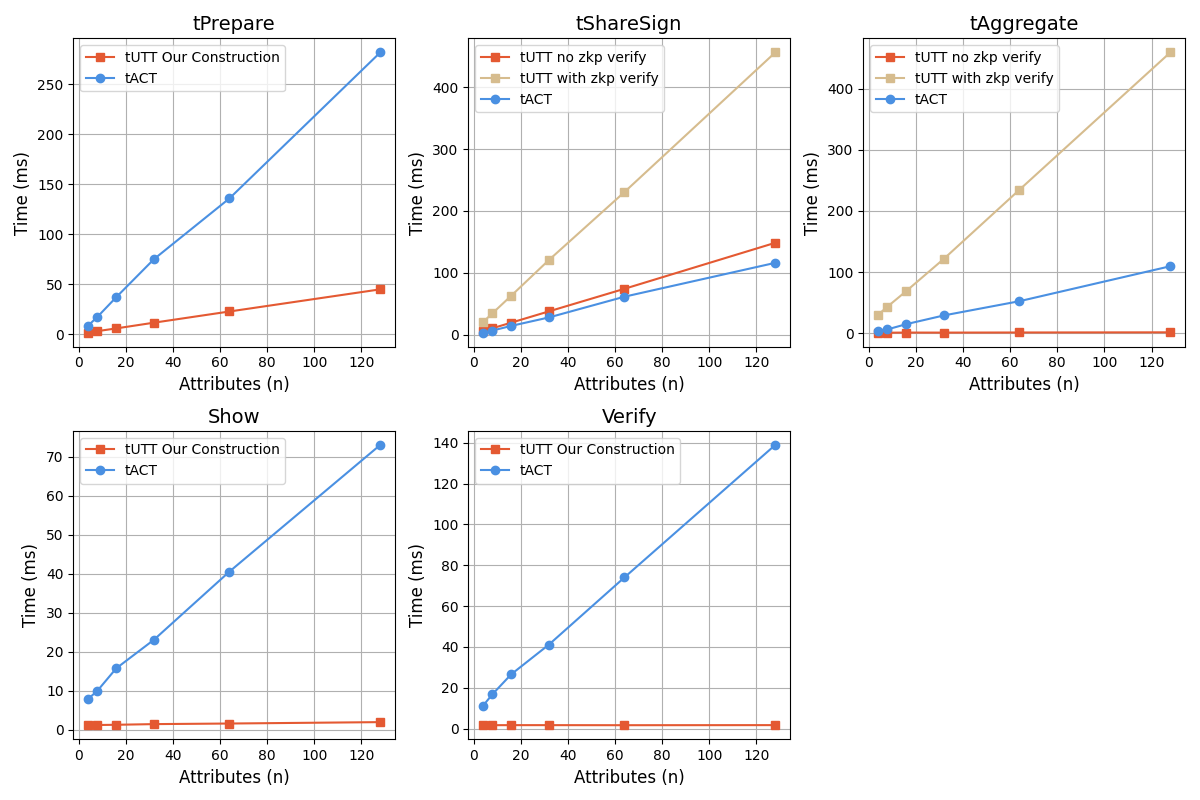
\includegraphics[width=0.9\linewidth]{figures/chap5_tutt_scale_by_n_attributes.png}
    \caption{Performance comparison when scaling by attribute count ($n$) with fixed $N=16, t=9$}
    \label{fig:chap5_tutt_scale_by_n}
    \vspace{-1em}
\end{figure}


\begin{itemize}
    \item \textbf{tPrepare (Commitment Generation):} Our construction significantly outperforms tACT, achieving $6.0\times$ faster operation at $n=64$ (22.71ms vs. 135.91ms). This advantage stems from our optimized multi-scalar multiplication (MSM) implementation in Schnorr proofs, allowing sublinear scaling with increasing attribute count.

    \item \textbf{tShareSign (Signature Share Generation):} This is the only operation where tACT outperforms our construction (61.34ms vs. 244.22ms at $n=64$), primarily because tACT doesn't perform zero-knowledge verification of its messages during signing, both for the issuer verifying from the user, and the user verifying the individual signature shares. For completeness, we present both with and without ZKP verification variants of our algorithm.

    \item \textbf{tAggregate (Signature Aggregation):} Our construction achieves  efficiency with $36.0\times$ speedup at $n=64$ (1.46ms vs. 52.55ms), we again leverage multi-scalar multiplication. 

    \item \textbf{Show and Verify:} These operations demonstrate our advantage with nearly constant-time performance regardless of attribute count. At $n=64$, our construction achieves $25.2\times$ speedup for Show (1.61ms vs. 40.56ms) and $44.1\times$ speedup for Verify (1.68ms vs. 74.07ms). This efficiency stems from our Schnorr ZKP approach, which avoids costly pairing checks per attribute or computing over $\G_T$ points.
\end{itemize}

The results in Figure~\ref{fig:chap5_tutt_scale_by_n} clearly illustrate how our construction maintains near-constant verification times regardless of attribute count, while tACT's performance degrades linearly with increasing attributes.


\subsubsection{Scaling with Threshold Size ($N$)}
We now examine performance with fixed attribute count ($n=16$) while varying threshold parameters across $N=4$ ($t=3$), $N=16$ ($t=9$), and $N=64$ ($t=33$). Key observations:



\begin{figure}[!htb]
    \centering
    \vspace{-0.5em}
    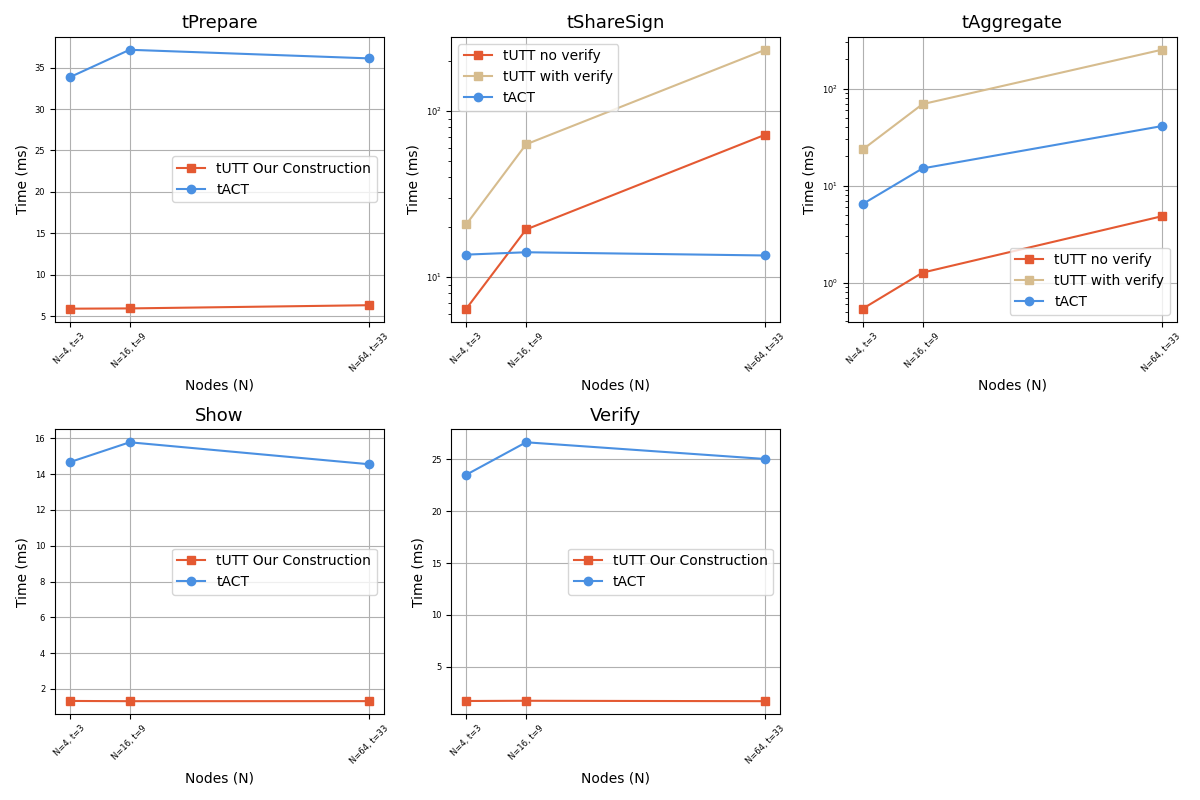
\includegraphics[width=0.9\linewidth]{figures/chap5_tutt_scale_by_N_nodes.png}
    \caption{Performance comparison when scaling by threshold size ($N$) with fixed $n=16$}
    \label{fig:chap5_tutt_scale_by_N}
    \vspace{-0.5em}
\end{figure}

\begin{itemize}
    \item \textbf{tShareSign Scalability:} Our construction's signing time increases with threshold size (21.19ms for $N=4$ to 283.72ms for $N=64$) due to our threshold key generation and signing approach. This contrasts with tACT's relatively stable performance ($\sim$13-14ms regardless of $N$).

    \item \textbf{Constant-Time Operations:} For user-centric operations (tPrepare, Show, Verify), our construction maintains excellent performance regardless of threshold size. Verify times remain approximately 1.7ms across all $N$ values, compared to tACT's $\sim$25ms.

    \item \textbf{Practical Implications:} These results suggest our construction is particularly well-suited for systems where credentials are frequently shown but rarely issued, as the verification performance advantage (up to $14.8\times$ at $N=64$) directly impacts end-user experience.
\end{itemize}


\begin{figure}[!htb]
    \centering
    \begin{minipage}[t]{0.48\textwidth}
        \centering
        
        \vspace{0.5em}
        \scriptsize
        \begin{tabular}{lccc}
        \toprule
        \textbf{Operation} & \textbf{n=4} & \textbf{n=16} & \textbf{n=64} \\
        \midrule
        tPrepare (Ours) & 1.65 & 6.16 & 22.71 \\
        Token Request & 8.55 & 37.15 & 135.91 \\
        \midrule
        tShareSign (Ours)$^{\dagger}$ & 20.95 & 63.40 & 244.22 \\
        Issue & 3.09 & 14.14 & 61.34 \\
        \midrule
        tAggregate (Ours) & 0.99 & 1.10 & 1.46 \\
        (Aggr., Unblind) & 3.92 & 15.04 & 52.55 \\
        \midrule
        Show (Ours) & 1.26 & 1.35 & 1.61 \\
        Prove & 7.90 & 15.78 & 40.56 \\
        \midrule
        Verify (Ours) & 1.71 & 1.82 & 1.68 \\
        Verify & 11.20 & 26.64 & 74.07 \\
        \bottomrule
        \end{tabular}
        \caption{tUTT (Ours) Performance scaling with attribute count ($n$) for fixed $N=16, t=9$ (ms) against tACT Construction}
        \label{tab:chap5_n_scaling_combined_utt_act}
    \end{minipage}
    \hfill
    \begin{minipage}[t]{0.48\textwidth}
        \centering
        
        \vspace{0.5em}
        \scriptsize
        \begin{tabular}{lccc}
        \toprule
        \textbf{Operation} & \textbf{N=4} & \textbf{N=16} & \textbf{N=64} \\
        \midrule
        tPrepare (Ours) & 5.97 & 6.16 & 5.88 \\
        Token Request & 33.84 & 37.15 & 36.11 \\
        \midrule
        tShareSign (Ours)$^{\dagger}$ & 21.19 & 63.40 & 283.72 \\
        Issue & 13.68 & 14.14 & 13.52 \\
        \midrule
        tAggregate (Ours) & 0.51 & 1.10 & 4.89 \\
        (Aggr., Unblind) & 6.46 & 15.04 & 41.02 \\
        \midrule
        Show (Ours) & 1.33 & 1.35 & 1.33 \\
        Prove & 14.67 & 15.78 & 14.55 \\
        \midrule
        Verify (Ours) & 1.69 & 1.82 & 1.69 \\
        Verify & 23.51 & 26.64 & 25.03 \\
        \bottomrule
        \end{tabular}
        \caption{tUTT (Ours)  Performance scaling with threshold size ($N$) for fixed $n=16$ (ms) against tACT Construction}
        \label{tab:N_scaling_combined_utt_act}
    \end{minipage}
    
    \vspace{-0.5em}
    \scriptsize
    % $^{\dagger}$ For this operation, TACT is faster than our construction.
\end{figure}


Figure~\ref{fig:chap5_tutt_scale_by_N} highlights the key trade-off in our design: while tShareSign performance scales less favorably with increasing threshold size, our user-centric operations (particularly Show and Verify) maintain consistently superior performance regardless of committee size.


\subsubsection{Performance Analysis Summary}
Our UTT (Ours) construction demonstrates superior performance in 4 out of 5 key operations, with notable advantages in:

\begin{enumerate}
    \item \textbf{Verification efficiency:} Near-constant verification time regardless of attribute count, critical for real-world deployment scenarios.

    \item \textbf{Show operation:} Consistently fast credential presentation (1.3-1.6ms), enabling responsive user experiences.

    \item \textbf{Attribute scalability:} Excellent performance with large attribute sets, allowing for richer credential schemas without performance penalties.
\end{enumerate}

The one trade-off is in signature share generation (tShareSign), where our construction prioritizes security through comprehensive zero-knowledge proofs at the cost of higher computational overhead. However, this operation typically occurs less frequently in practical deployments compared to verification operations.











\subsection{Threshold Identity System Evaluation}
\label{sec:threshold-performance}

We now analyze the complete T-SIRIS system's performance. Figure~\ref{fig:chap5_tsiris_performance} illustrates how each system operation scales with attribute count across different threshold configurations.

\begin{figure}[!htb]
    \centering
    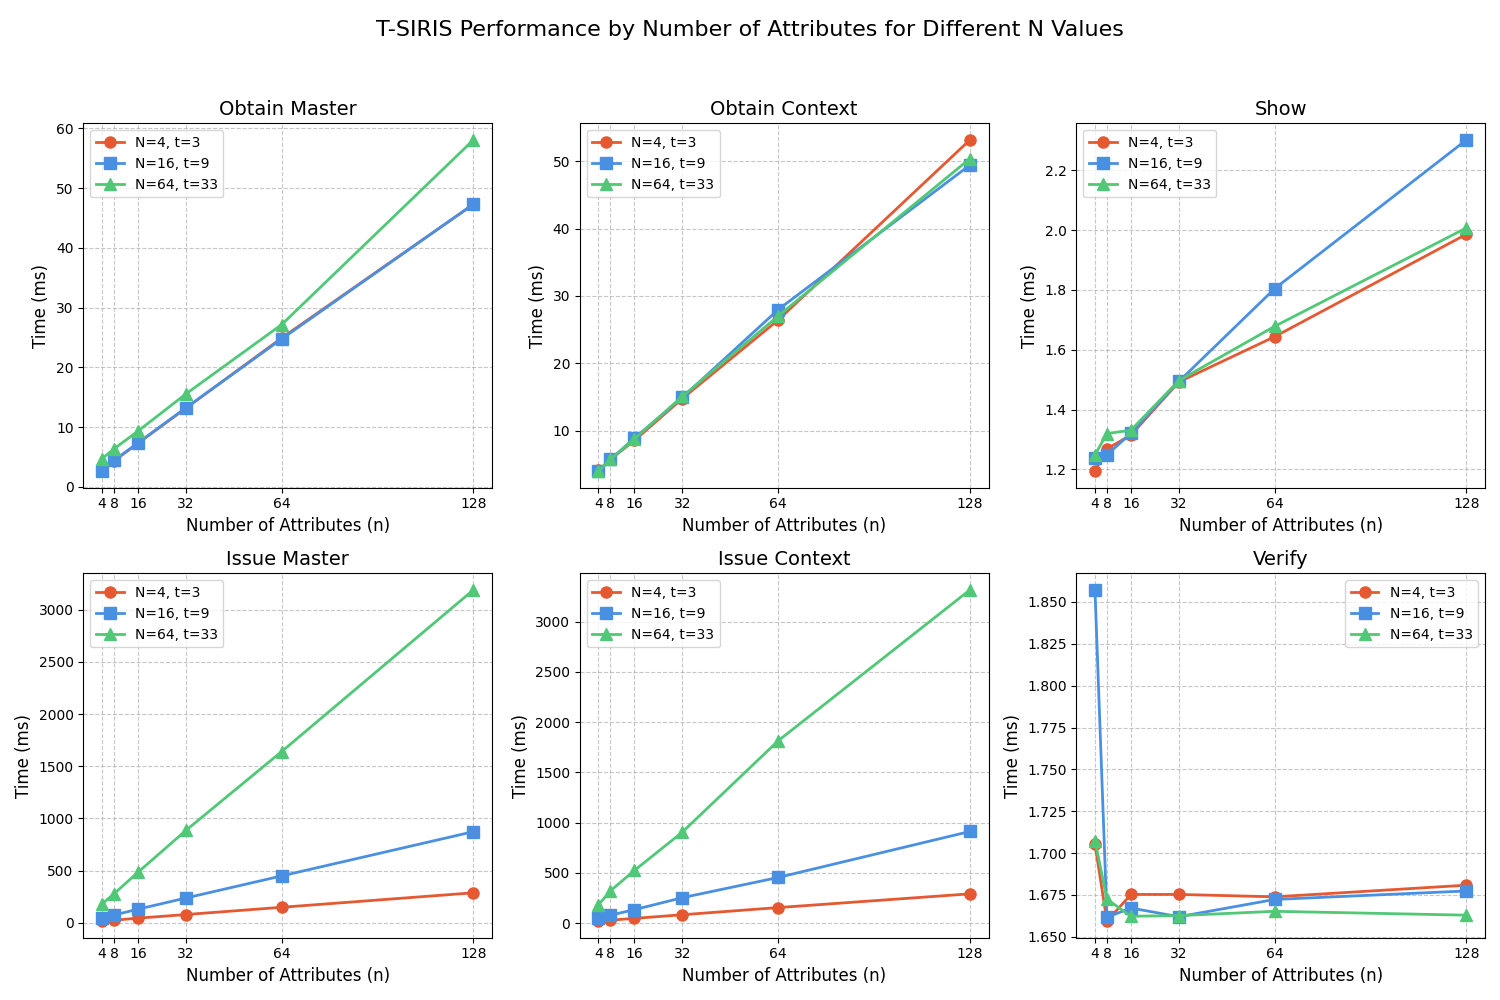
\includegraphics[width=\linewidth]{figures/chap5_tsiris_varyN_varyn_aggregate.png}
    \caption{T-SIRIS performance scaling with attribute count across operations}
    \label{fig:chap5_tsiris_performance}
\end{figure}

The results reveal several important characteristics of our system:

\begin{itemize}
    \item \textbf{User-side operations} (Obtain Master, Obtain Context, Show) scale linearly with attribute count, with Obtain Master at approximately $60ms$ for 128 attributes, enabling efficient user-side operation.
        
    \item \textbf{Issuer operations} (Issue Master, Issue Context) show notably different scaling behavior across threshold configurations. With 64 attributes, Issue Master takes approximately 200ms at N=4, 800ms at N=16, and 3000ms at N=64, highlighting the trade-off between decentralization and issuer-side performance. It's important to note that we do not issue with parallel computation and thus issuance time could be greatly reduced. We are opting for the worst-case scenario.
    
    \item \textbf{Verification operation} demonstrates near-constant time performance (approximately 1.7ms) regardless of attribute count or threshold configuration, crucial for high-throughput verification scenarios.

\end{itemize}

These measurements demonstrate that T-SIRIS achieves efficient credential presentation while maintaining acceptable issuance costs even with large threshold committees, making it practical for real-world deployment.


\subsection{Threshold Identity System Performance Comparison with S3ID}
 

\begin{figure}[!htb]
    \centering
    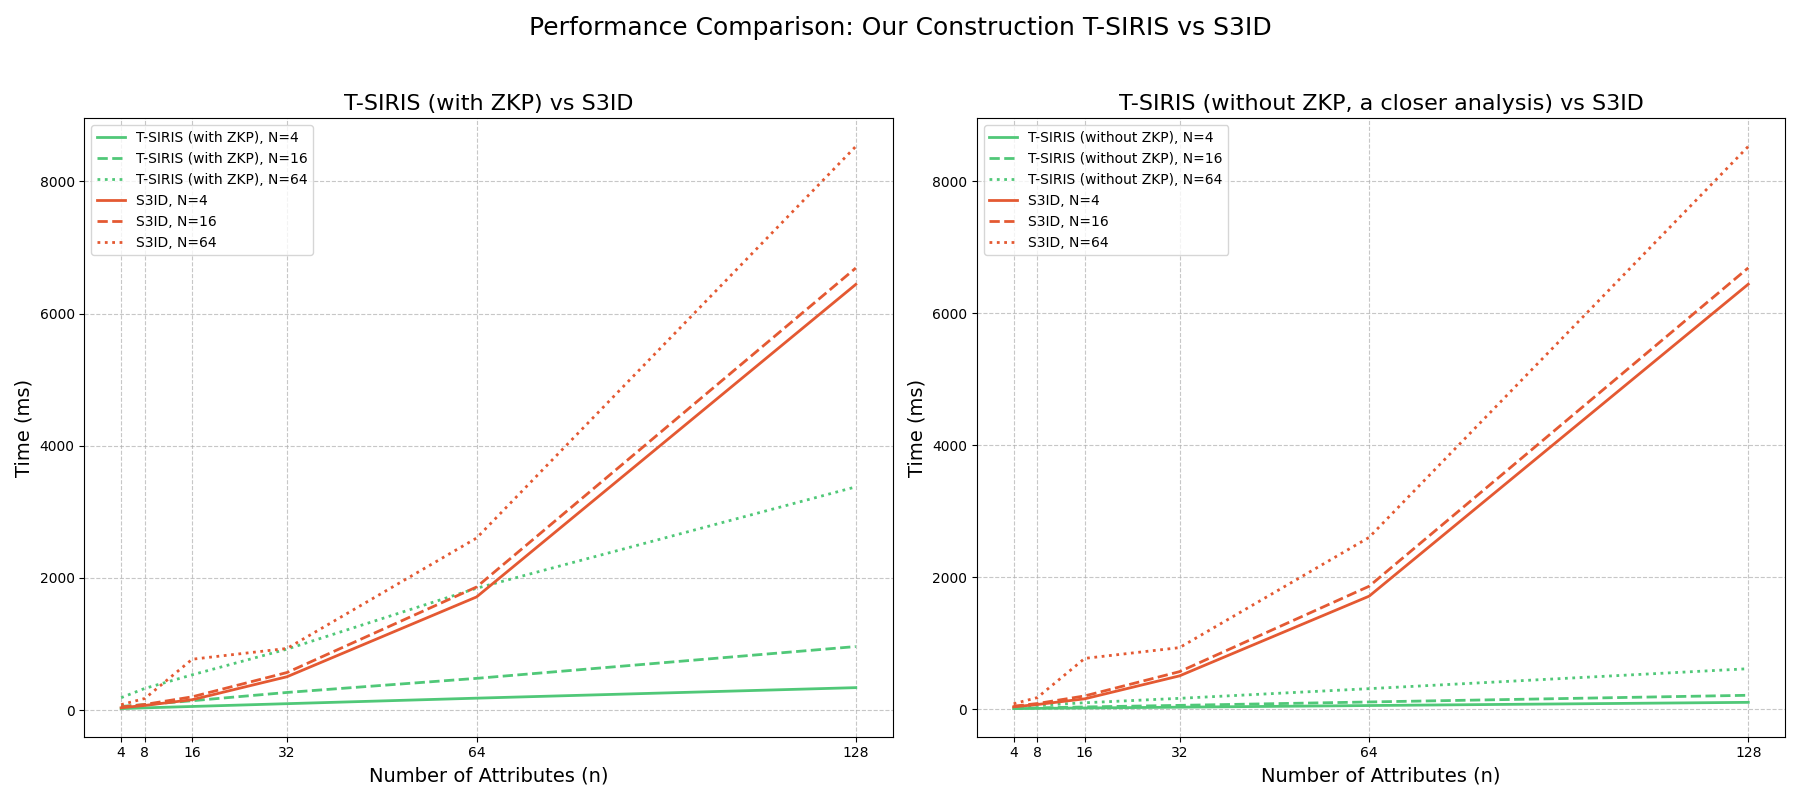
\includegraphics[width=\linewidth]{figures/chap5_tsiris_against_s3id.png}
    \caption{End-to-end performance comparison between T-SIRIS and S3ID}
    \label{fig:tsiris-vs-s3id}
\end{figure}


We present a performance comparison between T-SIRIS and S3ID. S3ID's algorithm Dedup combines the credential request and issuance process, with sybil resistance and verification. We combined our algorithm benchmarks to compare against this and plotted this figure: ~\ref{fig:tsiris-vs-s3id}.

The comparison reveals several significant advantages of our approach:

\begin{itemize}
    
    \item \textbf{Verification efficiency}: T-SIRIS maintains consistent sub-2ms verification time regardless of attribute count, while S3ID's verification time increases linearly, reaching approximately 25ms for just 16 attributes. This 12.5x improvement in verification throughput is critical for large-scale deployments.
    
    \item \textbf{Efficient Sybil resistance}: Our CRBN-based nullifier mechanism adds only 2.49ms overhead during credential issuance, approximately 5x faster than S3ID's token-based deduplication approach (12.8ms), while providing equivalent Sybil-resistance guarantees.
    
    \item \textbf{Scalable attribute support}: While both systems show linear scaling with attribute count, T-SIRIS demonstrates significantly better slopes across all operations, with the greatest advantage in verification operations (44.1x at 64 attributes).
\end{itemize}

Even when issuer-side ZKP verification is included (our full security model), T-SIRIS outperforms S3ID in end-to-end credential issuance and verification scenarios. The performance gap widens further at higher attribute counts, making T-SIRIS suitable for complex credential schemas with many attributes and verifying multiple credentials together.


